\documentclass[11]{article}
\usepackage{graphicx}
\graphicspath{ {images/} }


\title{CS2006 Python Project 1 - \\Classes and Iterators in Python}
\date{06/03/2018}
\author{Matriculation Numbers: 160001362, 160014817, 160013384 (Group 14)}

\begin{document}
	\maketitle
	\newpage
	\tableofcontents
	
	\newpage
	\section{Summary of Functionality}
		This practical specified the development of a mathematical system to explore discrete mathematical structures using the programming language Python. \\\\
The provided README file gives detailed instructions on what the solution can do and how to run each command. \\\\
The following functionality has been implemented:
	\subsection{Basic Specification:}
		All requirements from the basic specification have been implemented. They are as follows:	
		\begin{itemize}
			\item An implementation of the twisted integers data structure which supports addition and multiplication given by the following rules:
				\begin{itemize}
				\item a $\bigoplus$ b = (a + b) mod n 
				\item a $\bigotimes$ b = (a + b + a · b) mod n
				\end{itemize}
			\item Exceptions that are used to check that user input is valid.
		\end{itemize}
	
	\subsection{Additional Requirements:}
	 From the suggested additional requirements, all of the easy, medium and hard requirements have been implemented:
	 	\subsubsection{Easy}
			\begin{itemize}
				\item \textbf{Easy Requirement 1} - The function 'mulEqualToOne(n)' has been developed in the checker.py file which calculates for a given n all elements x $\epsilon$ Zn such that x $\bigotimes$ x = 1, where 1 $\epsilon$ Zn
				\item \textbf{Easy Requirement 2} - For a given n functions (in checker.py) have been developed to check whether the following properties hold for all x, y, z $\epsilon$ Zn (each of which returns a boolean signifying whether the properties hold):
				\begin{itemize}
					\item x $\bigoplus$ y = y $\bigoplus$ x - 'isCommutativeAdd(n)'
					\item x $\bigotimes$ y = y $\bigotimes$ x - 'isCommutativeMul(n)'
					\item (x $\bigoplus$ y) $\bigoplus$ z = x $\bigoplus$ (y $\bigoplus$ z) - 'isAssociativeAdd(n)'
					\item (x $\bigotimes$ y) $\bigotimes$ z = x $\bigotimes$ (y $\bigotimes$ z) - 'isAssociativeMul(n)'
					\item (x $\bigoplus$ y) $\bigotimes$ z = (x $\bigotimes$ y) $\bigoplus$ (y $\bigotimes$ z) - 'isDistributive(n)' \\\\ The first two of the above five functions have been optimised to avoid redundant checks.
				\end{itemize}
				
				\item \textbf{Easy Requirement 3} - The file twisted\_integers.py contains a class TwistedIntegers which implements a data structure representing Zn with respect to the operations a $\bigoplus$ b = (a $\bigoplus$ b) mod n and a $\bigotimes$ b = (a $\bigotimes$ b) mod n and contains the methods \_\_init\_\_, \_\_str\_\_ and size where size returns the number of elements in Zn.
			\end{itemize}

		\subsubsection{Medium}
			\begin{itemize}
				\item \textbf{Medium Requirement 1} - In the twisted\_integers.py file (along with the aforementioned TwistedIntegers class) the IteratorOfTwistedIntegers class has been implemented to iterate over instances of TwistedIntegers and contains an \_\_init\_\_ function (to initialise it with a given instance of TwistedIntegers), a hasNext() boolean function (to indicate if the iterator has a next value) and a next() function (to return the next value in the iterator).
				\item \textbf{Medium Requirement 2} - The function 'findValAdd(n)' in the twisted\_integers.py file finds for a given n all elements $\tau$ of Zn such that $\tau$ $\bigoplus$ x = x for all x $\epsilon$ Zn.
				\item \textbf{Medium Requirement 3} - The function 'findValMul(n)' in the twisted\_integers.py file finds for a given n all elements $\varepsilon$ of Zn such that $\varepsilon$ $\bigotimes$ x = x for all x $\epsilon$ Zn.
			\end{itemize}
		\subsubsection{Hard}
				\begin{itemize}
					\item \textbf{Hard Requirement 1} - In the twisted\_int\_matrix.py file the class TwistedIntMatrix has been implemented which represents a matrix of TwistedInt objects. The \_\_init\_\_ function of the class takes an x and y dimension as well as a list of TwistedInt objects and creates a matrix containing the values in the list. The \_\_mul\_\_ function implements matrix multiplication (between two given matrices) using the row by column rule and the $\bigoplus$ and $\bigotimes$ operators. This is achieved using the calcDotProduct function which calculates the dot product between a row and a column of the two matrices (which itself uses the getCol function to access a column of the second matrix). \\\\ For the same requirement, an algorithm has been implemented using the function getPossibleMatrices(matrices) which takes a list of M matrices and calculates all of the possible unique matrices that may be obtained by multiplying these matrices, i.e. the set  \{g1 ⊗ g2 ⊗ . . . ⊗ gk $\vert$ k $\epsilon$ N, gi $\epsilon$ M \}.
					\item \textbf{Hard Requirement 2} - The level of testing and documentation has been enhanced by including docstrings for every function and class, as well as example doctests within these docstrings that can be extracted and run to verify the correctness of the functions which they document.
				\end{itemize}
	\subsection{Further Features:}
		The follow additional features have also been implemented:
		\begin{itemize}
			\item An iterator class, IteratorOfTwistedIntMatrix, has been implemented in twisted\_int\_matrix.py file which iterates over an instance of TwistedIntMatrix from top left to bottom right across the TwistedInt elements. As with the IteratorOfTwistedIntegers iterator, this iterator has a hasNext(), next() and \_\_init\_\_ functions.
		\end{itemize}

	\section{Design and Implementation}
		\begin{itemize}
			\item \textbf{Basic Specification - TwistedInt Data Structure (twisted\_int.py)} - The TwistedInt data structure is implemented in twisted\_int.py. It is initialised by passing an integer value 'val' and mod value 'n' into \_\_init\_\_. The constructor of the TwistedInt class will raise a TypeError exception if 'val' or 'n' are not integers and will raise the custom InvalidModError or InvalidValError if the value of n passed in is less than 0 or if val is not in Zn, 0 to (n - 1). These exceptions can be handled by any implementing code to validate the inputs of the user. \\\\ The printing of TwistedInt objects has be modified in the function \_\_str\_\_ to printed TwistedInt instances in the format "$<$object:n$>$". \\\\ TwistedInt multiplication is implemented by the \_\_mul\_\_ function which takes two TwistedInts and compares their mod n values - raising a custom MismatchedModError exception if they are not equal - and otherwise performs the operation (a + b + a . b) mod n and assigns the result to the value of a new TwistedInt (as well as the same mod n value) and returns this object. \\\\ Similarly the \_\_add\_\_ function performs the operation (a + b) mod n with two given TwistedInt instances and returns a TwistedInt instance with the result as the integer value. 
			
			\item \textbf{Easy Requirements 1 and 2 (checker.py)} - The 'mulEqualToOne(n)' function implements easy requirement 1 of the specification. If the value of n passed into the function is either a string or is less than 0 then a TypeError exception or InvalidModError exception is raised respectively. If the value of n is valid then all possible values of x $\epsilon$ Zn are iterated over and checked to see whether the condition x $\bigotimes$ x = 1 holds. If the condition holds then the value of x is added to a list of valid ints which are returned at the end of the function. \\\\ For the second easy requirement each of the mathematical properties is tested using the respective functions isCommutativeAdd, isCommutativeMul, isAssociativeAdd, isAssociativeMul and isDistributive. Each of the functions iterate over all possible values of x, y, and z using for loops and evaluate their respective conditions. The first two functions (having only two variables to test) have been optimised to avoid redundant checks using the function combinations\_with\_replacement from the itertools from the Python standard library.
			
			\item \textbf{Easy Requirement 3 (twisted\_integers.py)} - The TwistedIntegers class implements the TwistedIntegers data structure that represents Zn for a given value of n. If the value n given is a string or is less than 0 then TypeError and InvalidModError exceptions are raised. Otherwise the class iterates over all possible values in Zn and assigns a TwistedInt instance for each into a list attribute. The \_\_str\_\_ function generates output of all the TwistedInt instances using the IteratorOfTwistedIntegers iterator implemented for Medium Requirement 1. The size function returns the value of n of the TwistedIntegers instance.
			
		\item \textbf{Medium Requirement 1 (twisted\_integer.py)} - The IteratorOfTwistedIntegers class implements the ability to iterate over a TwistedIntegers instance. The hasNext function in the iterator returns true if the current index of the iterator is less than the size of the TwistedIntegers instance in the iterator. The next function checks if the hasNext is false and if this is the case then an IndexError is raised. Otherwise the element at the current index is returned and the index of the iterator is incremented.
		
		\item \textbf{Medium Requirement 2 and 3 (twisted\_integers.py)} - The function findValAdd finds for a given n all elements $\tau$ of Zn such that $\tau$ $\bigoplus$ x = x for all x $\epsilon$ Zn. It does this by creating two IteratorOfTwistedIntegers instances and iterates over all values of $\tau$ in the outer loop and all possible values of x in the inner loop, each time checking whether the condition is true for those values of $\tau$ and x. If the condition holds for all values of x then the value of $\tau$ is added to a list of valid integers, otherwise the inner loop breaks to the outer loop. The list is returned at the end of the function. \\\\ Similarly using the same technique the function findValMul finds for a given n all elements $\varepsilon$ of Zn such that $\varepsilon$ $\bigotimes$ x = x for all x $\epsilon$ Zn.
		
		\item \textbf{Hard Requirement 1 (twisted\_int\_matrix.py)} - The TwistedIntMatrix class implements the functionality to create a matrix of TwistedInt instances by specifying an x dimension, y dimension and list of TwistedInts to populate the matrix. The constructor function for the class raises a custom MatrixIndexError exception if the size of the x or y dimensions are less than 0. It also raises a MatrixIndexError if the size of the matrix is smaller than the number of elements in the list of TwistedInts. Finally it throws as a MismatchedModError exception if not all of the TwistedInts  have the same mod value of n. If it is a valid instantiation then the class iterates over a matrix attribute and appends the values from the TwistedInt list to the correct index in the matrix. \\\\ The \_\_str\_\_ function allows the matrix to be printed as it uses an iterator to traverse the matrix and produce a string output of the elements within. \\\\ The \_\_mul\_\_ function allows traditional matrix row-column multiplication using the $\bigoplus$ and $\bigotimes$ operations. This is achieved by iterating over the matrices to be multiplied and calculating the dot product of each pair of rows and columns using the calcDotProduct function and the getCol functions. Appropriate exceptions are thrown (TypeError, ValueError and MismatchedModError) if the type of the second argument is not a matrix, the x and y dimensions of the matrices do not allow for multiplication, or the mod value of the two matrices are not equal, respectively. \\\\ The getPossibleMatrices function takes a list of matrices and uses the permutations function from itertools from the Python standard library to find all unique possible orderings of list indices for the matrix list. Each permutation is then iterated over and for each index in the permutation, the matrix at that index is accessed and multiplied by the following matrices in that same permutation. The result of this is added to a list of generated matrices.
		
		\item \textbf{Hard Requirement 2} - Extensive docStrings have been added to every function of the code. These can be seen inside the actual code, as well as inside the documentation folder, as HTML files. These also contain docTests - while not as extensive as unit testing, these provide an example of how to use  every function, and test that the basic functionality is correct. These can be run in the terminal. The outputs of running all these tests has been stored in docTest results.txt.		
		\end{itemize}
		
	\section{Evidence of Testing}	
		The code contains basic example docTests for every function. The output of which follows on the next page \footnote{Terminal output would have been directly included within this report rather than as a screen shot but the characters disagree with latex formatting}. The output of unit tests would have been displayed but as discussed in the Known Problems section, we could unfortunately not integrate them with the final implemenation. The results shown can also be found in results.txt. 
		\newpage
		
			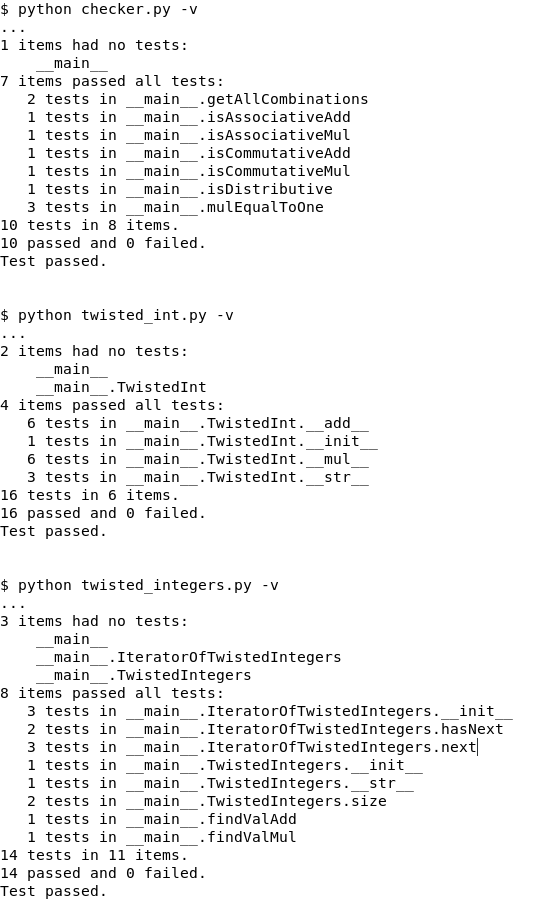
\includegraphics[scale=0.5]{Test1.png} \\\\
			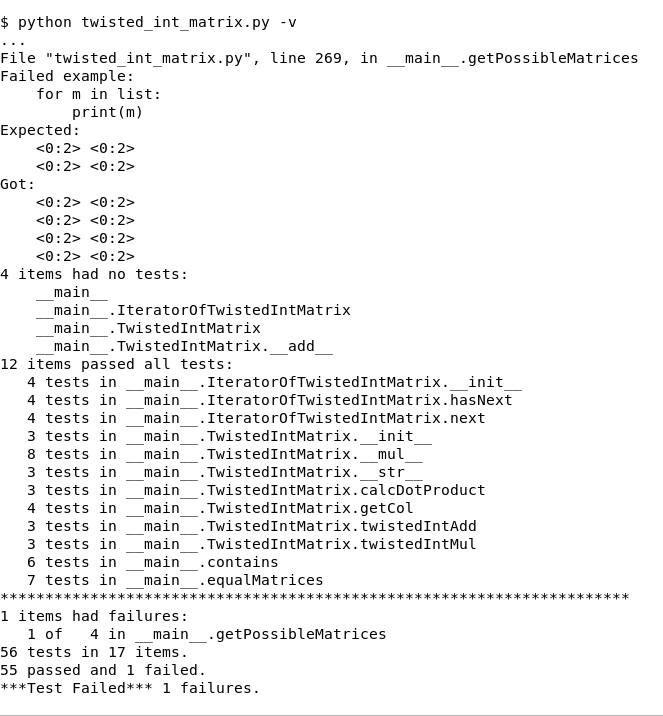
\includegraphics[scale=0.5]{Test2.png} \footnote{The 1 failure is the due to repeated results being printed due to a bug with the contains function when passing in the same matrix multiple times. This is discussed in the Known Problems section.}
		
	\section{Known Problems}
		For the algorithm of hard requirement 1 that aims to return a set of unique matrices produced as a result of multiplying a list of matrices in different permutations, the list of matrices produced contains repeated values when identical matrices are multiplied. This is because for some reason the contains function does not identify values that have already been added to the list of generated matrices correctly.
		
The unit tests are not correctly integrated with the system properly as they struggle to handle custom exceptions. They could also be more extensive. Therefore the only testing that successfully works is the docTesting from the second hard requirement.
		
	\section{Problems Overcome}
	Throughout the practical we overcame the challenge of working with multiple files in Python for the first time, as well as using docStrings and docTests with which we were unfamiliar. The implementation of the matrix functions were also challenging due to the extensive use of iteration but overall we managed to produce a working solution.

	\section{Summary of Provenance}
			\begin{itemize}
				\item 160001362:
					\begin{itemize}
						\item Basic Specification
						\item Easy Requirement 1
						\item Part of Easy Requirement 2
						\item Medium Requirement 2
						\item Medium Requirement 3
						\item Hard Requirement 1
					\end{itemize}
					
				\item 160012817:
					\begin{itemize}
						\item Part of Easy Requirement 2
						\item Easy Requirement 3
						\item Medium Requirement 1
						\item Hard Requirement 2
						\item General testing, validation (with exceptions) and maintenance.
					\end{itemize}
					
				\item 160013384: \footnote{Was sick for a week during development}
					\begin{itemize}
						\item Unit Testing 
					\end{itemize}
			\end{itemize}
				
	
\section{Conclusion}
	Overall, we have made a practical that we are proud of. All of the requirements are met (apart from testing extensively). Ideally we would have much better testing, but due to illness we were unable to include this in the practical. We have successfully got to grips with Python and created a working and well documented program.

\end{document}